\providecommand{\main}{..}
\documentclass[../mthe-493-final-project.tex]{subfiles}

% Tool identification & evaluation. Lay out all the "eng tools" we considered for a given section & make a case for each one. Determine which tools will be used too. Implementation and usage of selected tools in the next chapter
\begin{document}
    \chapter{Engineering Tools}
    \label{ch:engineering-tools}
    
    \section{Distributed Computing}
    \label{sec:distributed-computing-engineering-tools}
    
    \subsection{Requirements and Evaluation Framework}
    %% Predetermine how we are going to evaluate these tools
    To model the design problem and solution, appropriate tools are required. The tools discussed in this section will represent the distributed computing environment in isolation. The details of the optimization and federated learning tools will be expanded on in their respective sections, but baseline compatibility with the chosen framework will be crucial. Two aspects must be considered: the physical hardware to represent the different agents in the experimental setup, and the software framework that will manage the program flow. 
    
    The hardware used to serve as the learners must be relatively simple to setup, must be able to execute the tasks aligned with the application, and must have variable computational capacity to model heterogeneity. The hardware that will represent the orchestrator must be able to communicate with the learner via software means, and must be capable of aggregating the results from the parallel tasks.
    
    To facilitate the communication in the network, a framework is required to send and receive data. This network needs to be reliable, and effective at reporting detailed errors. To help this aspect, there should be a means of registering presence and identity of the learners. In other words, the orchestrator should know at any time how many learners are available for use, and should have a means of addressing each one directly. If a problem occurs during experimentation, such as losing connection to a learner, this should be clearly stated so that the experiment can be rerun or disregarded. The software will need to benchmark learners, send this data back to the orchestrator so that the optimization tools can be applied and the task load distribution can be determined. Then, the application software must be run on each of the learners, in this case: training a neural network. Metrics such as timing, model accuracy, total cost and benchmarking accuracy need to be recorded accurately and delivered to a central location for analysis post-experimentation. The results from the task execution on the various learners must then be aggregated, and the final results displayed. Additionally, the software used must be able to implement all of the problem constraints as specified. In particular, the way that learners charge a fee for performing a unit of work, and the granularity of control that the orchestrator uses to distribute tasks with cost considered must satisfy the requirements.
    
    For both the hardware and software tools, cost is an important factor to evaluate the options against. Hardware that must be purchased should be noted. For software, both the cost of licensing software that exists as well as the manpower cost of developing additional resources to support the framework needs to be weighed. 
    
    \subsection{Tools Explanation}
    %% Introduce tools to be evaluated
    The hardware considered to represent learners were Raspberry Pis and regular laptops/desktops. A Raspberry Pi is a small, minimal computer that is cheap to acquire and quick to setup. Regular laptops and desktops would be simple the personal computers that group members and  friends possess. 
    
    The software frameworks considered were Distributed Compute Protocol (DCP) from Kings Distributed Systems and Axon from this project's graduate collaborator Duncan Mays. DCP is a framework and business that lets users sign up to add their laptop to a global worker pool, where they can receive some money for having various parallelizable tasks run on their computers while they are idle. It is the foundation that underlies a successful business that has applications in the healthcare industry and in post-graduate research. Axon is a minimal framework that allows users to run experimental setups of distributed work. It is far more extensible given that it is minimal, but is not professionally supported.

    \subsection{Evaluation of Tools}
    \label{subsec-ete-evaluation-of-tools}
    %% Evaluate tools
    Raspberry Pis are relatively cheap and are easy to setup. They all have the same computational ability, however the CPUs can be overclocked at different rates to simulate heterogeneity in the learner pool. Without loss of generality, the laptops selected would have varying capacity across CPU clock speed, number of cores, amount of memory, and general architecture. This would provide a more natural variance across learners. A crucial make-or-break point of analysis was in the ability of the hardware to actually perform the federated learning tasks. Raspberry Pis were originally thought to be able to handle these tasks, but after a series of prototype attempts, it was concluded that they are essentially too minimal in their abilities and will produce unusable results from their work. A Raspberry Pi 4 B with 4GB of RAM costs \$75 per board, whereas devices that are already in the group's possession are free, so the latter will also be a more cost-effective solution~\cite{raspberry-pi-price}.
    
    Comparing DCP and Axon frameworks, one can look at the basic features. DCP is written in JavaScript, whereas Axon is written in Python. Both languages do not have much of a learning curve and both support machine learning libraries - TensorFlow for JavaScript and PyTorch for Python. DCP uses a custom network protocol for communication that is built on top of HTTP, whereas Axon uses Remote Procedure Call (RPC) to accomplish this feature. Both methods are effective and fault tolerant, however RPC does have a little more customization when it comes to timeout configurations. DCP is well supported by a business where Axon is supported solely by Duncan, though Duncan is very familiar with all aspects of the project. Both systems have a means of managing identity and presence, for DCP it is handled internally and is not user-facing, and in Axon a module called a notice board is available to meet this need. Neither system was initially set up to record metrics. On Axon, it was relatively trivial to implement these changes in an early prototype stage. With DCP, it was more difficult to dig in to the internals of how the system works to add these features manually, but the team was able to meet with the DCP owners to ask for these changes, and they were added in a timely manner. The critical requirement of being able to represent the fee-exchange system in a way that aligned with the problem specifications. The way that DCP fees work is the learner would set the minimum wage that they would be willing to receive, and the job deployer/orchestrator would set a fixed price that they are willing to pay. As long as the price meets or exceeds the minimum wage, then the learner is chosen for the job and all learners would be paid the same wage. The experimental setup requires learners to be able to be paid different wages that should be correlated to their efficacy at working. Cost is not implemented inherently in Axon, so there is a high degree of freedom. DCP does charge to use their framework with an average price of \$0.01435 per CPU-hour, whereas Axon is free to use~\cite{kings-ds-marketing}. However, Axon will need a lot more custom software built on top of it, and thus will require at least 40 hours of work, estimated at \$30/hr, resulting in approximately \$1200 of labour required to get the system to a usable state. 

    \section{Optimization}
    \label{sec:optimization-engineering-tools}
    
    % Write about SciPy linprog, PuLP, Gurobi, and heuristics in the same way as the presentation.
    
    The optimization problem as defined in \autoref{sec:optimization-problem-description} is a mixed integer programming (MIP) problem \cite{wolsey_mip}. As with other classes of mathematical programming problems, an \textit{optimization solver} is typically employed in the implementation of systems which require such problems to be solved. There are many such products, libraries, and resources that provide this functionality. These resources vary in scope, features, robustness; they may be open-source or closed-source, and commercial or freeware \cite{greenberg_nature_2010}. Most notably, libraries provide varying degrees of control over how a mathematical program may be specified, and (in the case of libraries providing multiple solver algorithms) which solver should be used to solve it.
    
    \subsection{Tool Criteria}
    \label{ssec:optimization-tool-criteria}
    
    Several criteria have been identified to allow a qualitative ranking of candidate solver libraries. This analysis will then be used to justify the selection of a solver library for further development of the project.
    
    On a side note, it is important to acknowledge that the constraint in \eqref{eq:optimization-constraint-3} (henceforth referred to as the \textit{beta constraint}) distinguishes this problem in difficulty from a standard MIP problem. Because of this, a portion of solver libraries will be unable to solve the problem as-stated, thus reducing the pool of candidate solvers from which to choose.
    
    The criteria that has been identified to evaluate candidate optimization solvers is listed below (in order of most-important to least-important), followed by an explanation of each criterion and their relative ranking of importance.
    
    \begin{enumerate}
        \item Efficacy in providing optimal solutions
        \item Algorithmic time complexity
        \item Ease of development
        \item Data privacy \& security
        \item Cost
    \end{enumerate}
    
    \textbf{Efficacy in providing optimal solutions} is an metric to assess whether a library is capable of providing feasible and optimal solutions to the optimization problem as defined in \autoref{sec:optimization-problem-description}. As mentioned above, optimization solver libraries vary in their scope, features, and robustness; not all libraries are capable of handling integrality constraints and/or the constraint in \eqref{eq:optimization-constraint-3}.
    This is selected as the primary criterion because a feasible and optimal solution to allocate data for minimal cost is paramount to the goals of the project. The selected solver and its implementation must be able to correctly identify the feasibility of a job given a set of learners and system parameters. It must then provide the minimum-cost allocation of data to learners.
    
    \textbf{Algorithmic time complexity} (running time) is the asymptotic behaviour of the solver's run time as the size of the input grows, commonly referred to as ``Big-O Notation''\cite{sipser_introduction_2013}. In this case, the `input size' is a combination of the size of the data set, $n$, and the number of learners available to the orchestrator, $k$. To deal with the varying levels of control libraries provide over the selection of algorithms, the running time will be assessed directly instead of a rigorous assessment of time complexity. A case-study MIP problem will be implemented in each library. The average running time of the case-study problem over a set of 10,000 input parameters will be calculated and used to rank candidates.
    This criterion is ranked second most-important because focus of the project on optimal data allocation \textit{under training time constraints}. The total execution time of the system includes network overhead, training overhead, and in particular, the orchestrator overhead. Orchestrator overhead includes the running time of the optimization solver. If this duration is minimized, more of the allotted time can be dedicated to training. In turn, this enlarges the feasible set by increasing the maximum quantity of work that can be completed by learners, $s^{max}_i$, in the allocated time $T$ (as defined in \autoref{sec:optimization-problem-description}). The larger enlarged feasible set may well contain the optimal solution. Therefore, it is of high priority that the optimization solver's running time is minimized.
    
    \textbf{Ease of development} is a qualitative metric that indicates how challenging it would be to implement a particular library into the project's code base. Some key components in this metric include
    \begin{itemize}
        \item ease of integration with the project's code base, written in the Python programming language \cite{10.5555/1593511},
        \item level of detail and completeness of library documentation (API specification, reference manuals, etc.), and
        \item availability of resources online (examples, tutorials, articles, etc.) A reliable proxy for this component is the number of weekly downloads from official sources.
    \end{itemize}
    This is the next most-important consideration because of time constraints on development efforts towards the project; it is not feasible to reverse-engineer a library's implementation given the duration and scope of this project.
    
    \textbf{Data privacy \& security} serves as an indication of the ethical implications of selecting a particular library through an assessment of how transparent and secure a given library is. Open-source libraries that contain no closed-source third-party code are very transparent regarding data privacy and data handling. When compared to their closed-source counterparts, open-source software projects are more secure and contain fewer vulnerabilities \cite{clarke2009open}. Additionally, closed-source projects are not required to disclose their data handling practices, which poses concerns about data privacy.
    This metric is important to consider due to the potential range of applications of this system in various industries. For example, medical research facilities may require the use of confidential patient information in the data set for a machine learning model. It is crucial that the confidentiality of this data is respected, as a security breach and/or mishandling of data would breach patient confidentiality and may have legal implications.
    
    \textbf{Cost} will be taken into account for all potential solutions. This is defined as any licensing or subscription fees, both for academic and commercial users. 
    This is an important metric because many optimization libraries are proprietary \cite{wikipedia_list_2011}, and the cost will be a factor in the project's economics.
    
    \subsection{Tool Evaluation}
    \label{ssec:optimization-tool-evaluation}
    
    Having identified four key criteria, four candidate optimization solvers were identified. In no particular order, they are
    \begin{itemize}
        \item SciPy
        \item PuLP
        \item Gurobi
        \item Heuristic Algorithm
    \end{itemize}
    All candidates satisfy the basic metric of having an interface with Python. The merits and flaws of each are now examined individually.
    
    \subsubsection{SciPy}
    \label{sssec:optimization-candidate-scipy}
    
    SciPy is a free, open-source scientific computing library for Python \cite{2020SciPy-NMeth}. It is popular, averaging over 1,000,000 downloads weekly \cite{flynn_2018_scipy}. Because of this popularity, there are many online resources for SciPy. Its documentation is also quite extensive, providing many examples and library use-cases.
    
    Included in SciPy is the \texttt{linprog} module, which supports a handful linear programming solvers (simplex, interior points methods, etc). The solvers in this library are well-optimized, taking advantage of pre-compiled binaries to accelerate their running time. This is in contrast to standard Python library, which is an interpreted language in its standard configuration.
    
    SciPy does not support MIP problems directly. This limitation can be resolved for some MIP problems through techniques such the \textit{relaxation} technique; however, the \textit{beta constraint} prohibits this technique from being employed in this project \cite{aps2020mosek}. For this reason, a SciPy-based solver implementation will not be feasible for this project, and it was excluded from the case-study MIP run-time comparison evaluation.
    
    \subsubsection{PuLP}
    \label{sssec:optimization-candidate-pulp}
    
    PuLP is a free, open-source collection of LP and MIP solvers for Python \cite{Mitchell11pulp}. It is significantly less popular than SciPy, averaging only 20,000 downloads weekly \cite{flynn_2018_pulp}. This naturally leads to fewer community resources available online. The documentation is not as extensive as that of SciPy either, furthering hindering the ease of development.
    
    PuLP's support for MIP problems makes it more robust than SciPy; when leveraging the simplifications in \autoref{ssec:optimization-problem-simplification}, PuLP is be able to implement a solver for the project's optimization problem.
    
    PuLP takes a unique approach in its method of distributing solvers supported by the library. Some solvers included rely on third-party packages, which do not come with the PuLP library. Some of these are closed-source and require additional licensing and fees, whilst others are operating-system dependent native libraries. This poses a data privacy and security risk \cite{clarke2009open}, and introduces uncertainty in solver running time depending on the availability of third-party packages in the end-user's system.
    
    When the case-study MIP problem was implemented in PuLP, the average solver running time was 32.5 seconds over the sample of 10,000 randomly-generated input parameters.
    
    \subsubsection{Gurobi}
    \label{sssec:optimization-candidate-gurobi}
    
    Gurobi is a proprietary, closed-source optimization library with support for Python \cite{gurobi}. It is distributed for academic and commercial uses, and requires a license and special installation routine. Because of the special installation routine, there are no available metrics on the the popularity of Gurobi. However, Gurobi's website claims over 2400 companies subscribe to their commercial license, including some Fortune 500 companies (Ibid.) Gurobi provides extensive documentation on their programming interfaces in addition to a official forum for community users, so there are plenty of available resources to aid in development. Ease of development is only hindered by the installation routine.
    
    Gurobi offers the most robust set of features, with support for LP, MIP, and more complex mathematical programming problems. They support linear, quadratic, and \textit{general} constraints (e.g. \texttt{min}, \texttt{max}). Hence, the library of optimization solvers provided by Gurobi is more substantial than SciPy and PuLP, and is more than capable of solving the optimization problem in this project.
    
    Because Gurobi is strictly closed-source, there is no method of validating the data handling practices and/or security vulnerabilities present in their optimization solvers. This poses a data privacy and security risk to using Gurobi \cite{clarke2009open}.
    
    Gurobi provides its academic license free-of-charge to all users belonging to an academic institution. However, commercial users are required to purchase a license. Research suggests that the quoted price can vary wildly depending on client use-case and scale, but some sources suggest a license may cost upwards of \$12,000 USD for a single-user license \cite{collart_cloud_2016}.
    
    When the case-study MIP problem was implemented in Gurobi, the average solver running time was 8.4 seconds over the sample of 10,000 randomly-generated input parameters. This demonstrates a speedup of approximately four-times when compared to PuLP.
    
    \subsubsection{Heuristic Algorithm}
    \label{sssec:optimization-candidate-heuristic}
    
    A heuristic algorithm (in the context of optimization solvers) is any algorithm which solves an optimization problem using unconventional methods that are generally specific to a single or subset of optimization problems. They are generally faster, at the expense of precision, optimality, or completeness of the solutions they generate \cite{kenny_heuristic_2014}.
    
    A heuristic algorithm can be developed to solve the project optimization problem as-stated in \autoref{sec:optimization-problem-description}. This would require more development time and resources than any previous library, because a successful algorithm would need to be formulated, implemented, and validated. To guarantee the correctness/optimality of solutions, one may implement the optimization problem through alternative means with a traditional optimization solver and compare the results. Furthermore, the optimality of a heuristic algorithm would require a rigorous mathematical proof.
    
    A heuristic algorithm would be developed entirely in-house for the project. This means the data privacy and security concerns that arise with traditional optimization solver libraries are not a concern; the data is handled entirely within the project, without the need for third-party involvement.
    
    The usage of a custom heuristic algorithm would not contribute any additional costs to the project's economics.
    
    The running time of a heuristic algorithm is entirely dependent on the specific algorithm in question, which, in turn, relies solely on the nature of the optimization problem at hand. Thus, the superiority of running times under a heuristic algorithm in a case-study MIP problem does not imply that heuristic algorithms will always be superior to traditional solvers. Nonetheless, a heuristic algorithm was developed for the case-study MIP problem for the sake of completeness. The algorithm averaged a running time of 3.7 seconds over an identical sample of 10,000 randomly-generated input parameters. This was more than a two-fold improvement over Gurobi's run-time average, and nearly nine-fold improvement over that of PuLP.
    
    \subsection{Tool Selection}
    \label{ssec:optimization-tool-selection}
    
    The evaluation results from \autoref{ssec:optimization-tool-evaluation} are summarized in \autoref{tab:optimization-tool-summary}.
    \begin{table}
        \begin{tabular}{| c || c c c c c |}
            \hline
            Candidate & Efficacy & Running Time & Development & Privacy & Cost \\ [0.5ex] 
            \hline\hline
            SciPy & Infeasible & N/A & Easy & Great & Free \\ 
            \hline
            PuLP & Optimal & Slow & Medium & Adequate & Free \\
            \hline
            Gurobi & Optimal & Fast & Easy & Poor & Proprietary \\
            \hline
            \textbf{Heuristic} & \textbf{Feasible} & \textbf{Varies} & \textbf{Hard} & \textbf{Great} & \textbf{Free} \\
            \hline
        \end{tabular}
        \caption{\label{tab:optimization-tool-summary}Summary of optimization solver candidate performance}
    \end{table}
    After evaluating the tools on the basis of the aforementioned criteria, SciPy was disqualified as a candidate because it does not meet the minimum efficacy criterion.
    
    PuLP was a strong candidate for all criteria except for running time. Because running time was identified as the second-most-important criterion, it was determined that PuLP will not be an effective optimization solver for the purposes of this project.
    
    The heuristic algorithm was identified as having the highest potential of all candidates, subject to additional risks. It is feasible that a heuristic algorithm may provide optimal solutions, but this cannot be guaranteed in advance of development. Additionally, the running time could vary greatly depending on the specific algorithm and its implementation.
    
    To account for these risks, the runner-up candidate, Gurobi, will be developed in parallel to a heuristic algorithm. The Gurobi implementation will serve as an alternative to validate both the correctness of solutions and compare running time of the heuristic algorithm. In the event that an algorithm cannot be developed, or if the heuristic implementation is not as effective as the Gurobi implementation, the project will continue with the Gurobi implementation as the primary optimization solver.
    
    \section{Parallel Learning}
    \label{sec:parallel-learning-engineering-tools}
    When approaching our parallel learning problem, much alike any other machine learning or deep learning problem, the best tools usually already exist. The field is booming with research and even in niche applications, it’s difficult to beat out the resources and personnel of FAANG research. With this in mind, the tools we’ll evaluate for our model aggregation problem will be three state of the art papers from Federated Learning. This is the area of distributed learning receiving the most research and thus the best model aggregation techniques come from federated papers as opposed to parallel papers.

    The first paper is commonly known as FedAvg but was formally titled Communication Efficient Learning of Deep Networks from Decentralized Data by Google research. In the FedAvg paper, edge devices range from smartphones to laptops to surveillance cameras. The paper details much of the data collection and preparation associated with federated learning, but this is not of our concern. It’s the impressively simple yet sophisticated aggregation algorithm that motivated our evaluation of this paper. The FedAvg algorithm is detailed in figure.
    \begin{figure}
        \centering
        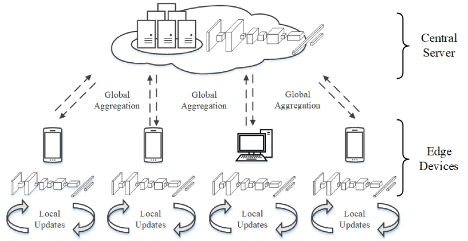
\includegraphics[width=115mm,scale=0.35]{thesis/img/tool_eval_1.png}
        \caption{FedAvg Network Communication}
        \label{fig:FedAvg}
    \end{figure}

    It begins by selecting a random fraction of clients to receive the current global model from the central server. These chosen edge devices perform local training where it’s explicitly stipulated that stochastic gradient descent is used as an optimizer. After local training is completed, model parameters are uploaded to the central server for aggregation. The aggregation algorithm computes weights for each edge device based upon the size of the dataset that was used in training. With these weights, an update to the global model is calculated by taking a weighted average of all the local updates \cite{FedAvg}.

    FedAvg represents the gold standard in model aggregation as this algorithm highly accurately mimics single device training. Further tool evaluation will only be performed to ensure that a niche version of FedAvg with edge case consideration favourable for this project doesn’t exist.
    The next two papers represent exactly this, FedAvg spin offs with specific edge case considerations. To avoid egregious repetition, the basic central server and edge device set up remains more or less identical and the learners are all given weights based upon dataset size. 
    
    Next, we’ll look at FedProx or Federated Optimization in Heterogeneous Networks by Facebook research. In their own words it’s a “generalization and re-parametrization of FedAvg”. FedProx aims to tackle overfitting and offer expedited convergence. The difference in Facebook’s approach to FedProx is the introduction of a penalization system. Learners with the most drastic changes on a given local update will have their weight reduced to diminish their influence over the global update. FedProx’s main advantage over FedAvg comes in highly heterogeneous settings where it demonstrates more stable and accurate convergence \cite{FedProx}.
    
    The final paper to be evaluated is q-FedAvg or Fair Resource Allocation in Federated Learning by Facebook AI \& CMU. q-FedAvg represents a combination of techniques from FedAvg and FedProx. This time the introduction of a penalization system takes aim at accuracy. Learners with lower ranking chosen accuracy metrics will have their weights reduced to diminish their influence of the subsequent global update. q-FedAvg’s main advantage over FedAvg comes in efficiency where the number of global cycles to convergence can be drastically reduced in optimal conditions \cite{q-FedAvg}.
    
    The final area of tool evaluation for our parallel learning application is typical machine learning. However, as was stipulated in the problem description, this is not a machine learning based problem, but instead an optimization problem with model aggregation as the application. For this reason, things like network architecture, loss functions, optimizers, learning rates, \& more have all been kept constant \& we’ve avoided using training techniques like dropout, batch normalization, and data augmentation. This was all done in an attempt to standardize our results so the focus could fall on finding the optimal dataset partition \& aggregating model parameters. What this did for our experimental results was set a ceiling on how accurate the network could get when the challenge of model aggregation was non-existent.
    
    The only typical machine learning tool to be evaluated in our experimentation is weight initialization. This clearly has a direct impact on our problem as the first global update comes from local models trained from base weights and biases. The three initialization techniques that will be considered are known as xavier uniform, kaiming uniform [better known as ‘he initialization’], and orthogonal in PyTorch. Xavier and kaiming both represent bounded Gaussian distributions whereas orthogonal represents a technique where the resulting model is semi-orthogonal. They will be tested on our set of learners for an optimal initialization scheme specific to our project.

\end{document}